% Options for packages loaded elsewhere
\PassOptionsToPackage{unicode}{hyperref}
\PassOptionsToPackage{hyphens}{url}
\PassOptionsToPackage{dvipsnames,svgnames,x11names}{xcolor}
%
\documentclass[
  letterpaper,
  DIV=11,
  numbers=noendperiod]{scrartcl}

\usepackage{amsmath,amssymb}
\usepackage{iftex}
\ifPDFTeX
  \usepackage[T1]{fontenc}
  \usepackage[utf8]{inputenc}
  \usepackage{textcomp} % provide euro and other symbols
\else % if luatex or xetex
  \usepackage{unicode-math}
  \defaultfontfeatures{Scale=MatchLowercase}
  \defaultfontfeatures[\rmfamily]{Ligatures=TeX,Scale=1}
\fi
\usepackage{lmodern}
\ifPDFTeX\else  
    % xetex/luatex font selection
\fi
% Use upquote if available, for straight quotes in verbatim environments
\IfFileExists{upquote.sty}{\usepackage{upquote}}{}
\IfFileExists{microtype.sty}{% use microtype if available
  \usepackage[]{microtype}
  \UseMicrotypeSet[protrusion]{basicmath} % disable protrusion for tt fonts
}{}
\makeatletter
\@ifundefined{KOMAClassName}{% if non-KOMA class
  \IfFileExists{parskip.sty}{%
    \usepackage{parskip}
  }{% else
    \setlength{\parindent}{0pt}
    \setlength{\parskip}{6pt plus 2pt minus 1pt}}
}{% if KOMA class
  \KOMAoptions{parskip=half}}
\makeatother
\usepackage{xcolor}
\setlength{\emergencystretch}{3em} % prevent overfull lines
\setcounter{secnumdepth}{-\maxdimen} % remove section numbering
% Make \paragraph and \subparagraph free-standing
\ifx\paragraph\undefined\else
  \let\oldparagraph\paragraph
  \renewcommand{\paragraph}[1]{\oldparagraph{#1}\mbox{}}
\fi
\ifx\subparagraph\undefined\else
  \let\oldsubparagraph\subparagraph
  \renewcommand{\subparagraph}[1]{\oldsubparagraph{#1}\mbox{}}
\fi

\usepackage{color}
\usepackage{fancyvrb}
\newcommand{\VerbBar}{|}
\newcommand{\VERB}{\Verb[commandchars=\\\{\}]}
\DefineVerbatimEnvironment{Highlighting}{Verbatim}{commandchars=\\\{\}}
% Add ',fontsize=\small' for more characters per line
\usepackage{framed}
\definecolor{shadecolor}{RGB}{241,243,245}
\newenvironment{Shaded}{\begin{snugshade}}{\end{snugshade}}
\newcommand{\AlertTok}[1]{\textcolor[rgb]{0.68,0.00,0.00}{#1}}
\newcommand{\AnnotationTok}[1]{\textcolor[rgb]{0.37,0.37,0.37}{#1}}
\newcommand{\AttributeTok}[1]{\textcolor[rgb]{0.40,0.45,0.13}{#1}}
\newcommand{\BaseNTok}[1]{\textcolor[rgb]{0.68,0.00,0.00}{#1}}
\newcommand{\BuiltInTok}[1]{\textcolor[rgb]{0.00,0.23,0.31}{#1}}
\newcommand{\CharTok}[1]{\textcolor[rgb]{0.13,0.47,0.30}{#1}}
\newcommand{\CommentTok}[1]{\textcolor[rgb]{0.37,0.37,0.37}{#1}}
\newcommand{\CommentVarTok}[1]{\textcolor[rgb]{0.37,0.37,0.37}{\textit{#1}}}
\newcommand{\ConstantTok}[1]{\textcolor[rgb]{0.56,0.35,0.01}{#1}}
\newcommand{\ControlFlowTok}[1]{\textcolor[rgb]{0.00,0.23,0.31}{#1}}
\newcommand{\DataTypeTok}[1]{\textcolor[rgb]{0.68,0.00,0.00}{#1}}
\newcommand{\DecValTok}[1]{\textcolor[rgb]{0.68,0.00,0.00}{#1}}
\newcommand{\DocumentationTok}[1]{\textcolor[rgb]{0.37,0.37,0.37}{\textit{#1}}}
\newcommand{\ErrorTok}[1]{\textcolor[rgb]{0.68,0.00,0.00}{#1}}
\newcommand{\ExtensionTok}[1]{\textcolor[rgb]{0.00,0.23,0.31}{#1}}
\newcommand{\FloatTok}[1]{\textcolor[rgb]{0.68,0.00,0.00}{#1}}
\newcommand{\FunctionTok}[1]{\textcolor[rgb]{0.28,0.35,0.67}{#1}}
\newcommand{\ImportTok}[1]{\textcolor[rgb]{0.00,0.46,0.62}{#1}}
\newcommand{\InformationTok}[1]{\textcolor[rgb]{0.37,0.37,0.37}{#1}}
\newcommand{\KeywordTok}[1]{\textcolor[rgb]{0.00,0.23,0.31}{#1}}
\newcommand{\NormalTok}[1]{\textcolor[rgb]{0.00,0.23,0.31}{#1}}
\newcommand{\OperatorTok}[1]{\textcolor[rgb]{0.37,0.37,0.37}{#1}}
\newcommand{\OtherTok}[1]{\textcolor[rgb]{0.00,0.23,0.31}{#1}}
\newcommand{\PreprocessorTok}[1]{\textcolor[rgb]{0.68,0.00,0.00}{#1}}
\newcommand{\RegionMarkerTok}[1]{\textcolor[rgb]{0.00,0.23,0.31}{#1}}
\newcommand{\SpecialCharTok}[1]{\textcolor[rgb]{0.37,0.37,0.37}{#1}}
\newcommand{\SpecialStringTok}[1]{\textcolor[rgb]{0.13,0.47,0.30}{#1}}
\newcommand{\StringTok}[1]{\textcolor[rgb]{0.13,0.47,0.30}{#1}}
\newcommand{\VariableTok}[1]{\textcolor[rgb]{0.07,0.07,0.07}{#1}}
\newcommand{\VerbatimStringTok}[1]{\textcolor[rgb]{0.13,0.47,0.30}{#1}}
\newcommand{\WarningTok}[1]{\textcolor[rgb]{0.37,0.37,0.37}{\textit{#1}}}

\providecommand{\tightlist}{%
  \setlength{\itemsep}{0pt}\setlength{\parskip}{0pt}}\usepackage{longtable,booktabs,array}
\usepackage{calc} % for calculating minipage widths
% Correct order of tables after \paragraph or \subparagraph
\usepackage{etoolbox}
\makeatletter
\patchcmd\longtable{\par}{\if@noskipsec\mbox{}\fi\par}{}{}
\makeatother
% Allow footnotes in longtable head/foot
\IfFileExists{footnotehyper.sty}{\usepackage{footnotehyper}}{\usepackage{footnote}}
\makesavenoteenv{longtable}
\usepackage{graphicx}
\makeatletter
\def\maxwidth{\ifdim\Gin@nat@width>\linewidth\linewidth\else\Gin@nat@width\fi}
\def\maxheight{\ifdim\Gin@nat@height>\textheight\textheight\else\Gin@nat@height\fi}
\makeatother
% Scale images if necessary, so that they will not overflow the page
% margins by default, and it is still possible to overwrite the defaults
% using explicit options in \includegraphics[width, height, ...]{}
\setkeys{Gin}{width=\maxwidth,height=\maxheight,keepaspectratio}
% Set default figure placement to htbp
\makeatletter
\def\fps@figure{htbp}
\makeatother

\KOMAoption{captions}{tableheading}
\makeatletter
\makeatother
\makeatletter
\makeatother
\makeatletter
\@ifpackageloaded{caption}{}{\usepackage{caption}}
\AtBeginDocument{%
\ifdefined\contentsname
  \renewcommand*\contentsname{Table of contents}
\else
  \newcommand\contentsname{Table of contents}
\fi
\ifdefined\listfigurename
  \renewcommand*\listfigurename{List of Figures}
\else
  \newcommand\listfigurename{List of Figures}
\fi
\ifdefined\listtablename
  \renewcommand*\listtablename{List of Tables}
\else
  \newcommand\listtablename{List of Tables}
\fi
\ifdefined\figurename
  \renewcommand*\figurename{Figure}
\else
  \newcommand\figurename{Figure}
\fi
\ifdefined\tablename
  \renewcommand*\tablename{Table}
\else
  \newcommand\tablename{Table}
\fi
}
\@ifpackageloaded{float}{}{\usepackage{float}}
\floatstyle{ruled}
\@ifundefined{c@chapter}{\newfloat{codelisting}{h}{lop}}{\newfloat{codelisting}{h}{lop}[chapter]}
\floatname{codelisting}{Listing}
\newcommand*\listoflistings{\listof{codelisting}{List of Listings}}
\makeatother
\makeatletter
\@ifpackageloaded{caption}{}{\usepackage{caption}}
\@ifpackageloaded{subcaption}{}{\usepackage{subcaption}}
\makeatother
\makeatletter
\@ifpackageloaded{tcolorbox}{}{\usepackage[skins,breakable]{tcolorbox}}
\makeatother
\makeatletter
\@ifundefined{shadecolor}{\definecolor{shadecolor}{rgb}{.97, .97, .97}}
\makeatother
\makeatletter
\makeatother
\makeatletter
\makeatother
\ifLuaTeX
  \usepackage{selnolig}  % disable illegal ligatures
\fi
\IfFileExists{bookmark.sty}{\usepackage{bookmark}}{\usepackage{hyperref}}
\IfFileExists{xurl.sty}{\usepackage{xurl}}{} % add URL line breaks if available
\urlstyle{same} % disable monospaced font for URLs
\hypersetup{
  pdftitle={homework 3},
  colorlinks=true,
  linkcolor={blue},
  filecolor={Maroon},
  citecolor={Blue},
  urlcolor={Blue},
  pdfcreator={LaTeX via pandoc}}

\title{homework 3}
\author{}
\date{}

\begin{document}
\maketitle
\ifdefined\Shaded\renewenvironment{Shaded}{\begin{tcolorbox}[boxrule=0pt, breakable, borderline west={3pt}{0pt}{shadecolor}, sharp corners, frame hidden, enhanced, interior hidden]}{\end{tcolorbox}}\fi

\hypertarget{getting-started}{%
\subsection{Getting Started}\label{getting-started}}

\begin{Shaded}
\begin{Highlighting}[]
\FunctionTok{library}\NormalTok{(dplyr)}
\FunctionTok{library}\NormalTok{(ggplot2)}
\FunctionTok{library}\NormalTok{(readr)}
\FunctionTok{library}\NormalTok{(tidytext)}
\FunctionTok{library}\NormalTok{(tidyverse)}
\NormalTok{data }\OtherTok{\textless{}{-}} \FunctionTok{read\_csv}\NormalTok{(}\StringTok{"https://raw.githubusercontent.com/USCbiostats/data{-}science{-}data/master/03\_pubmed/pubmed.csv"}\NormalTok{)}
\end{Highlighting}
\end{Shaded}

\begin{Shaded}
\begin{Highlighting}[]
\FunctionTok{head}\NormalTok{(data)}
\end{Highlighting}
\end{Shaded}

\begin{verbatim}
# A tibble: 6 x 2
  abstract                                                                 term 
  <chr>                                                                    <chr>
1 "Background and aims: Many patients with coronavirus disease 2019 (COVI~ covid
2 "Introduction: Contradictory data have been reported on the incidence o~ covid
3 "This article aims at collecting all information needed for dentists re~ covid
4 "OBJECTIVE. The objective of our study was to determine the misdiagnosi~ covid
5 "Background: Much of the focus regarding the global pandemic of coronav~ covid
6 "The World Health Organization (WHO) has issued a warning that, althoug~ covid
\end{verbatim}

\begin{Shaded}
\begin{Highlighting}[]
\FunctionTok{tail}\NormalTok{(data)}
\end{Highlighting}
\end{Shaded}

\begin{verbatim}
# A tibble: 6 x 2
  abstract                                                                 term 
  <chr>                                                                    <chr>
1 From Antenatal Diagnostic Center referrals over 22 months, consultation~ pree~
2 Objective: To describe the duration of expectant management and the ind~ pree~
3 Objective: To examine the effect of a combination of screening and trea~ pree~
4 Objective: To assess obstetric outcomes in women in their second pregna~ pree~
5 Preeclampsia is a pregnancy-associated illness affecting multiple organ~ pree~
6 Eighty-eight normotensive gravid women between 24 and 34 weeks of gesta~ pree~
\end{verbatim}

\hypertarget{question-1}{%
\section{Question 1}\label{question-1}}

\begin{Shaded}
\begin{Highlighting}[]
\NormalTok{data }\SpecialCharTok{|\textgreater{}} \FunctionTok{unnest\_tokens}\NormalTok{(}\AttributeTok{output=}\NormalTok{word, }\AttributeTok{input=}\NormalTok{abstract) }\SpecialCharTok{|\textgreater{}}
  \FunctionTok{anti\_join}\NormalTok{(stop\_words, }\AttributeTok{by =} \FunctionTok{c}\NormalTok{(}\StringTok{"word"}\NormalTok{)) }\SpecialCharTok{|\textgreater{}}
  \FunctionTok{count}\NormalTok{(word, }\AttributeTok{sort =} \ConstantTok{TRUE}\NormalTok{) }\SpecialCharTok{|\textgreater{}}
  \FunctionTok{top\_n}\NormalTok{(}\DecValTok{20}\NormalTok{, n)}
\end{Highlighting}
\end{Shaded}

\begin{verbatim}
# A tibble: 20 x 2
   word             n
   <chr>        <int>
 1 covid         7275
 2 19            7080
 3 patients      4674
 4 cancer        3999
 5 prostate      3832
 6 disease       2574
 7 pre           2165
 8 eclampsia     2005
 9 preeclampsia  1863
10 treatment     1841
11 clinical      1682
12 risk          1588
13 women         1327
14 study         1299
15 results       1281
16 severe        1063
17 diagnosis     1015
18 pregnancy     1011
19 data           945
20 health         922
\end{verbatim}

\begin{Shaded}
\begin{Highlighting}[]
\NormalTok{data }\SpecialCharTok{|\textgreater{}} \FunctionTok{unnest\_tokens}\NormalTok{(word, abstract) }\SpecialCharTok{|\textgreater{}}
  \FunctionTok{count}\NormalTok{(word, }\AttributeTok{sort =} \ConstantTok{TRUE}\NormalTok{) }\SpecialCharTok{|\textgreater{}}
  \FunctionTok{top\_n}\NormalTok{(}\DecValTok{20}\NormalTok{, n)}
\end{Highlighting}
\end{Shaded}

\begin{verbatim}
# A tibble: 20 x 2
   word         n
   <chr>    <int>
 1 the      28126
 2 of       24760
 3 and      19993
 4 in       14653
 5 to       10920
 6 a         8245
 7 with      8038
 8 covid     7275
 9 19        7080
10 is        5649
11 for       5492
12 patients  4674
13 cancer    3999
14 prostate  3832
15 was       3315
16 that      3226
17 were      3226
18 as        3159
19 this      3158
20 are       2833
\end{verbatim}

\hypertarget{question-2}{%
\section{Question 2}\label{question-2}}

\begin{Shaded}
\begin{Highlighting}[]
\NormalTok{bigrams }\OtherTok{\textless{}{-}}\NormalTok{ data }\SpecialCharTok{\%\textgreater{}\%}
  \FunctionTok{unnest\_ngrams}\NormalTok{(ngram, abstract, }\AttributeTok{n =} \DecValTok{2}\NormalTok{) }

\NormalTok{bigrams }\SpecialCharTok{\%\textgreater{}\%}
  \FunctionTok{count}\NormalTok{(ngram, }\AttributeTok{sort =} \ConstantTok{TRUE}\NormalTok{) }\SpecialCharTok{\%\textgreater{}\%}
  \FunctionTok{top\_n}\NormalTok{(}\DecValTok{10}\NormalTok{, n) }\SpecialCharTok{\%\textgreater{}\%}
  \FunctionTok{ggplot}\NormalTok{(}\FunctionTok{aes}\NormalTok{(n, }\FunctionTok{fct\_reorder}\NormalTok{(ngram, n))) }\SpecialCharTok{+}
  \FunctionTok{geom\_col}\NormalTok{()}
\end{Highlighting}
\end{Shaded}

\begin{figure}[H]

{\centering 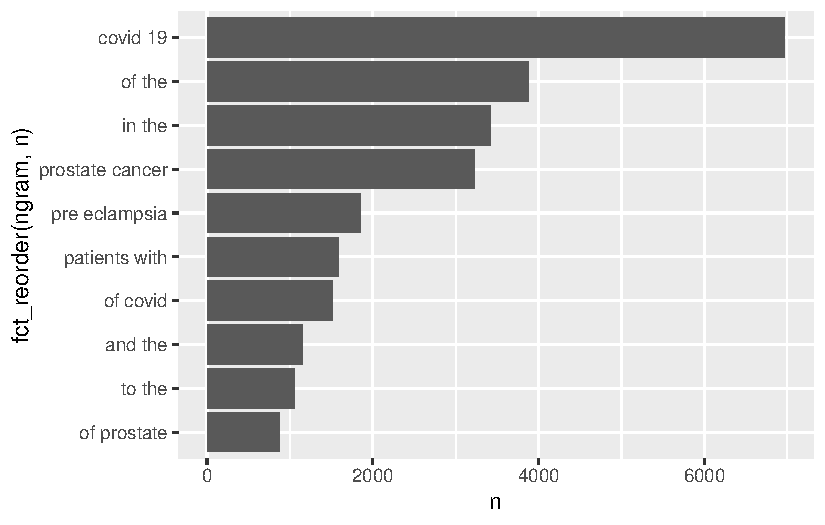
\includegraphics{hw3_files/figure-pdf/unnamed-chunk-4-1.pdf}

}

\end{figure}

\hypertarget{question-3}{%
\section{Question 3}\label{question-3}}

\begin{Shaded}
\begin{Highlighting}[]
\NormalTok{numbers\_df }\OtherTok{\textless{}{-}} \FunctionTok{data.frame}\NormalTok{(}\AttributeTok{word=}\FunctionTok{as.character}\NormalTok{(}\DecValTok{0}\SpecialCharTok{:}\DecValTok{50}\NormalTok{))}

\NormalTok{results }\OtherTok{\textless{}{-}}\NormalTok{ data }\SpecialCharTok{|\textgreater{}} \FunctionTok{unnest\_tokens}\NormalTok{(}\AttributeTok{output=}\NormalTok{word, }\AttributeTok{input=}\NormalTok{abstract)}\SpecialCharTok{|\textgreater{}}
  \FunctionTok{anti\_join}\NormalTok{(stop\_words, }\AttributeTok{by =} \FunctionTok{c}\NormalTok{(}\StringTok{"word"}\NormalTok{)) }\SpecialCharTok{|\textgreater{}}
  \FunctionTok{anti\_join}\NormalTok{(numbers\_df, }\AttributeTok{by =} \FunctionTok{c}\NormalTok{(}\StringTok{"word"}\NormalTok{)) }\SpecialCharTok{|\textgreater{}}
  \FunctionTok{count}\NormalTok{(word, term) }\SpecialCharTok{|\textgreater{}}
  \FunctionTok{bind\_tf\_idf}\NormalTok{(}\AttributeTok{term=}\NormalTok{word, }\AttributeTok{document=}\NormalTok{term, }\AttributeTok{n=}\NormalTok{n) }\SpecialCharTok{|\textgreater{}}
  \FunctionTok{group\_by}\NormalTok{(term) }\SpecialCharTok{|\textgreater{}}
  \FunctionTok{top\_n}\NormalTok{(}\AttributeTok{n=}\DecValTok{5}\NormalTok{, }\AttributeTok{wt=}\NormalTok{tf\_idf) }\SpecialCharTok{|\textgreater{}}
  \FunctionTok{arrange}\NormalTok{(}\FunctionTok{desc}\NormalTok{(tf\_idf)) }\SpecialCharTok{|\textgreater{}}
  \FunctionTok{ungroup}\NormalTok{() }\SpecialCharTok{|\textgreater{}}
  \FunctionTok{arrange}\NormalTok{(term)}

\FunctionTok{print}\NormalTok{(}\AttributeTok{n=}\DecValTok{50}\NormalTok{, results)}
\end{Highlighting}
\end{Shaded}

\begin{verbatim}
# A tibble: 25 x 6
   word            term                n      tf   idf  tf_idf
   <chr>           <chr>           <int>   <dbl> <dbl>   <dbl>
 1 covid           covid            7275 0.0706  1.61  0.114  
 2 pandemic        covid             800 0.00776 1.61  0.0125 
 3 coronavirus     covid             647 0.00628 1.61  0.0101 
 4 sars            covid             372 0.00361 1.61  0.00581
 5 cov             covid             334 0.00324 1.61  0.00521
 6 cf              cystic fibrosis   625 0.0239  0.916 0.0219 
 7 fibrosis        cystic fibrosis   867 0.0331  0.511 0.0169 
 8 cystic          cystic fibrosis   862 0.0329  0.511 0.0168 
 9 cftr            cystic fibrosis    86 0.00329 1.61  0.00529
10 sweat           cystic fibrosis    83 0.00317 1.61  0.00511
11 meningitis      meningitis        429 0.0170  1.61  0.0274 
12 meningeal       meningitis        219 0.00869 1.61  0.0140 
13 pachymeningitis meningitis        149 0.00591 1.61  0.00952
14 csf             meningitis        206 0.00817 0.916 0.00749
15 meninges        meningitis        106 0.00421 1.61  0.00677
16 eclampsia       preeclampsia     2005 0.0262  1.61  0.0422 
17 preeclampsia    preeclampsia     1863 0.0244  1.61  0.0392 
18 pregnancy       preeclampsia      969 0.0127  0.511 0.00648
19 maternal        preeclampsia      797 0.0104  0.511 0.00533
20 gestational     preeclampsia      191 0.00250 1.61  0.00402
21 prostate        prostate cancer  3832 0.0571  1.61  0.0919 
22 androgen        prostate cancer   305 0.00454 1.61  0.00731
23 psa             prostate cancer   282 0.00420 1.61  0.00676
24 prostatectomy   prostate cancer   215 0.00320 1.61  0.00515
25 castration      prostate cancer   148 0.00220 1.61  0.00355
\end{verbatim}



\end{document}
